\documentclass{article}
\usepackage[a4paper, margin=2cm]{geometry}
\usepackage{xcolor}
\usepackage{xspace}
\usepackage{booktabs}
\usepackage{dsfont}
\usepackage{footmisc}
\usepackage{marvosym}
\usepackage{amsmath}
\usepackage{hyperref}
\usepackage[capitalise,noabbrev]{cleveref}
\usepackage{tabularx}
\usepackage{listings}
\usepackage{multirow}
\usepackage{pgfplots}
\pgfplotsset{compat=newest}

\usepgfplotslibrary{groupplots}
\pgfplotsset{every axis/.style={scale only axis}}

\pgfplotsset{
  % Mark repeat, but the last mark is always drawn
  mark repeat*/.style={
    scatter,
    scatter src=x,
    scatter/@pre marker code/.code={
      \pgfmathtruncatemacro\usemark{
        or(mod(\coordindex,#1)==0, (\coordindex==(\numcoords-1))
      }
      \ifnum\usemark=0
        \pgfplotsset{mark=none}
      \fi
    },
    scatter/@post marker code/.code={}
  },
  log x ticks with fixed point/.style={
      xticklabel={
        \pgfkeys{/pgf/fpu=true}
        \pgfmathparse{exp(\tick)}%
        \pgfmathprintnumber[fixed relative, precision=3]{\pgfmathresult}
        \pgfkeys{/pgf/fpu=false}
      }
  },
  log y ticks with fixed point/.style={
      yticklabel={
        \pgfkeys{/pgf/fpu=true}
        \pgfmathparse{exp(\tick)}%
        \pgfmathprintnumber[fixed relative, precision=3]{\pgfmathresult}
        \pgfkeys{/pgf/fpu=false}
      }
  },
  major grid style={thin,dotted},
  minor grid style={thin,dotted},
  ymajorgrids,
  yminorgrids,
  every axis/.append style={
    line width=0.7pt,
    tick style={
      line cap=round,
      thin,
      major tick length=4pt,
      minor tick length=2pt,
    },
    mark options={solid},
  },
  legend cell align=left,
  legend style={
    line width=0.7pt,
    /tikz/every even column/.append style={column sep=3mm,black},
    /tikz/every odd column/.append style={black},
    mark options={solid},
  },
  % move title closer
  legend style={font=\small},
  title style={yshift=-2pt},
  % less space on left and right
  enlarge x limits=0.04,
  every tick label/.append style={font=\footnotesize},
  every axis label/.append style={font=\small},
  every axis y label/.append style={yshift=-1ex},
  /pgf/number format/1000 sep={},
  axis lines*=left,
  xlabel near ticks,
  ylabel near ticks,
  axis lines*=left,
  label style={font=\footnotesize},
  tick label style={font=\footnotesize},
  width=65mm,
  height=55mm,
  log x ticks with fixed point,
}

\definecolor{veryLightGrey}{HTML}{F2F2F2}
\definecolor{lightGrey}{HTML}{DDDDDD}
\definecolor{colorSimdRecSplit}{HTML}{444444}
\definecolor{colorChd}{HTML}{377EB8}
\definecolor{colorRustFmph}{HTML}{A65628}
\definecolor{colorRustFmphGo}{HTML}{A65628}
\definecolor{colorRustPHast}{HTML}{FF5733}
\definecolor{colorSicHash}{HTML}{4DAF4A}
\definecolor{colorPthash}{HTML}{984EA3}
\definecolor{colorDensePtHash}{HTML}{377EB8}
\definecolor{colorRecSplit}{HTML}{FF7F00}
\definecolor{colorBbhash}{HTML}{F781BF}
\definecolor{colorShockHash}{HTML}{F8BA01}
\definecolor{colorBipartiteShockHash}{HTML}{F781BF}
\definecolor{colorBipartiteShockHashFlat}{HTML}{E41A1C}
\definecolor{colorBmz}{HTML}{000000}
\definecolor{colorBdz}{HTML}{444444}
\definecolor{colorFch}{HTML}{444444}
\definecolor{colorChm}{HTML}{A65628}
\definecolor{colorFiPS}{HTML}{FF7F00}
\definecolor{colorConsensus}{HTML}{4DAF4A}
\definecolor{colorPtrHash}{HTML}{F8BA01}
\definecolor{colorMorphisHash}{HTML}{A65628}
\definecolor{colorMorphisHashFlat}{HTML}{E41A1C}

\title{MPHF plot}
\date{}
\begin{document}

% IMPORT-DATA competitorNames _competitorNames.txt
% IMPORT-DATA inputData dominance-map.txt
% SQL DELETE FROM inputData WHERE threads != 1 OR loadFactor != 1.0
% SQL DELETE FROM inputData WHERE name = "PartitionedPTHash"
% SQL DELETE FROM inputData WHERE constructionTimeMilliseconds > 5000000

%%%%%%%%%%%%%%%%%%%%%%%%% Pareto plots %%%%%%%%%%%%%%%%%%%%%%%%%

% SQL CREATE TABLE paretoConstruction AS SELECT * FROM inputData
%% SQL DELETE FROM paretoConstruction
%%     WHERE EXISTS (SELECT * FROM paretoConstruction other WHERE other.name = paretoConstruction.name
%%             AND other.bitsPerElement <= paretoConstruction.bitsPerElement
%%             AND other.constructionTimeMilliseconds <= paretoConstruction.constructionTimeMilliseconds
%%             AND (other.bitsPerElement < bitsPerElement
%%               OR other.constructionTimeMilliseconds < paretoConstruction.constructionTimeMilliseconds))

% SQL CREATE TABLE paretoQuery AS SELECT * FROM inputData
%% SQL DELETE FROM paretoQuery
%%     WHERE EXISTS (SELECT * FROM paretoQuery other WHERE other.name = paretoQuery.name
%%             AND other.bitsPerElement <= paretoQuery.bitsPerElement
%%             AND other.queryTimeMilliseconds <= paretoQuery.queryTimeMilliseconds
%%             AND (other.bitsPerElement < bitsPerElement
%%               OR other.queryTimeMilliseconds < paretoQuery.queryTimeMilliseconds))

%%%%%%%%%%%%%%%%%%%%%%%% Dominance Maps %%%%%%%%%%%%%%%%%%%%%%%% 

% SQL CREATE TABLE dominanceMap AS SELECT * FROM inputData
% Remove hopelessly bad measurements to clean up plots
%% SQL DELETE FROM dominanceMap
%% WHERE EXISTS (SELECT * FROM dominanceMap other WHERE
%%     other.bitsPerElement < dominanceMap.bitsPerElement
%%     AND other.constructionTimeMilliseconds < dominanceMap.constructionTimeMilliseconds
%%     AND other.queryTimeMilliseconds < dominanceMap.queryTimeMilliseconds)

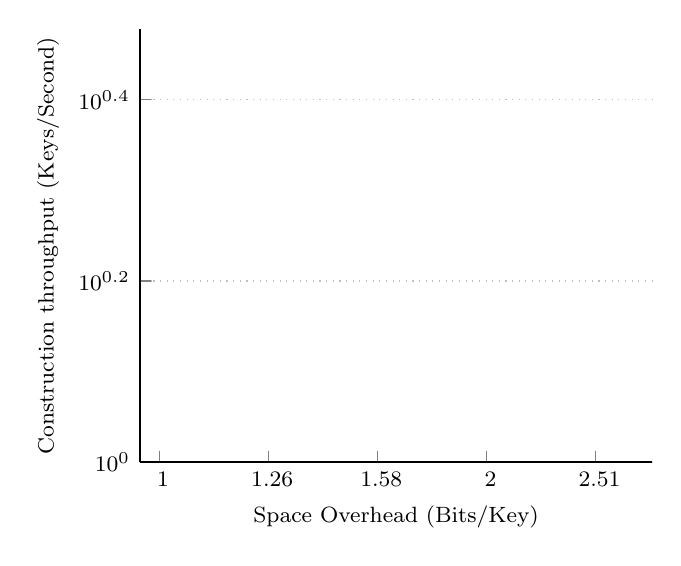
\begin{tikzpicture}
    \begin{axis}[
            ylabel={Construction throughput (Keys/Second)},
            xlabel={Space Overhead (Bits/Key)},
            xmode=log,
            ymode=log,
            legend columns=4,
            legend to name=legend,
            xmin=0.015,
            xmax=5,
            ymin=1e4,
        ]
        %% MULTIPLOT(name|ptitle|attr)
        %% SELECT
        %%    bitsPerElement-1.4427 as x,
        %%    1000.0*N/constructionTimeMilliseconds as y,
        %%    store_attr || IIF(name LIKE "%PTHash" OR name LIKE "%SicHash" OR name LIKE "ShockHash%", ",mark repeat*=4", "") as attr,
        %%    IFNULL(store_name, "name" || " !! missing from competitorNames.txt") as ptitle,
        %%    MULTIPLOT
        %% FROM paretoConstruction
        %% LEFT JOIN competitorNames ON name = store_code
        %% ORDER BY store_name,name,x,y
    \end{axis}
\end{tikzpicture}
%
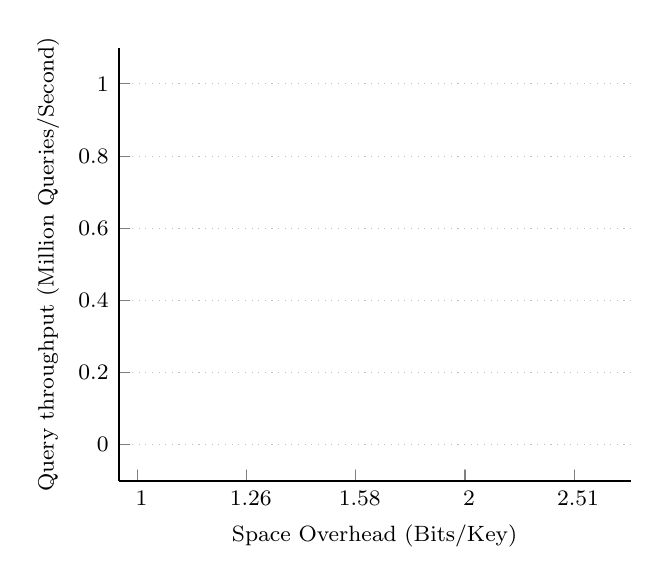
\begin{tikzpicture}
    \begin{axis}[
            ylabel={Query throughput (Million Queries/Second)},
            xlabel={Space Overhead (Bits/Key)},
            xmode=log,
            xmin=0.015,
            xmax=5,
        ]
        %% MULTIPLOT(name|ptitle|attr|nolegend)
        %% SELECT
        %%    bitsPerElement-1.4427 as x,
        %%    0.001*numQueries/queryTimeMilliseconds as y,
        %%    store_attr as attr,
        %%    IFNULL(store_name, "name" || " !! missing from competitorNames.txt") as ptitle,
        %%    MULTIPLOT
        %% FROM paretoQuery
        %% LEFT JOIN competitorNames ON name = store_code
        %% ORDER BY store_name,name,x,y
    \end{axis}
\end{tikzpicture}

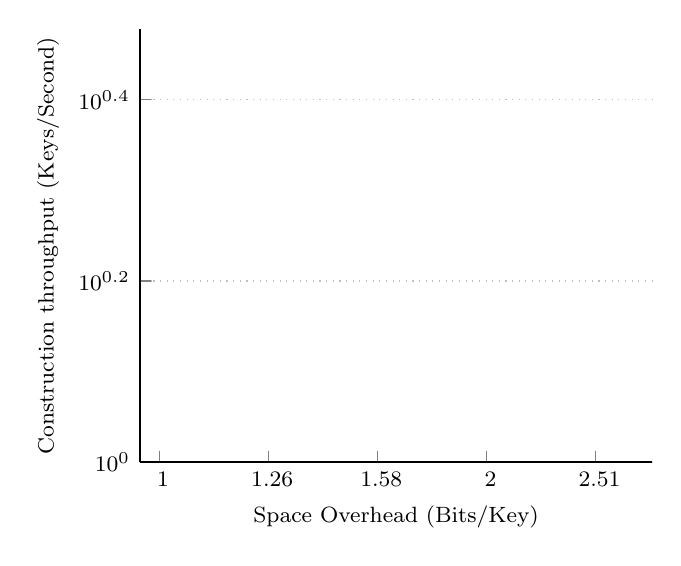
\begin{tikzpicture}
    \begin{axis}[
            ylabel={Construction throughput (Keys/Second)},
            xlabel={Space Overhead (Bits/Key)},
            xmode=log,
            ymode=log,
            patch,
            patch type=rectangle,
            shader=flat,
            xmin=0.015,
            xmax=5,
            ymin=1e4,
        ]
        % Each point in the dominance map is a rectangle going infinitely far to the right and bottom.
        % Sorting the draw order of these rectangles by the third dimension gives the dominance map.
        % The NULL values in the rectangle get filled with the actual measurements.
        % Given that the y axis is logarithmic (therefore, there is no y=0), we stop each rectangle at 1e4
        % SQL CREATE TABLE rectangle (rectangleX INT, rectangleY INT)
        % SQL INSERT INTO rectangle VALUES (NULL,NULL),(10,NULL),(10,1e4),(NULL,1e4)

        %% MULTIPLOT(ptitle|attr|nolegend)
        %% SELECT
        %%   IFNULL(rectangleX, bitsPerElement-1.4427) AS x,
        %%   IFNULL(rectangleY, 1000.0*N/constructionTimeMilliseconds) AS y,
        %%   store_attr || ",solid,mark=none,line width=0" AS attr,
        %%   store_name as ptitle
        %% FROM dominanceMap
        %% CROSS JOIN rectangle
        %% LEFT JOIN competitorNames ON name = store_code
        %% ORDER BY queryTimeMilliseconds DESC
    \end{axis}
\end{tikzpicture}
%
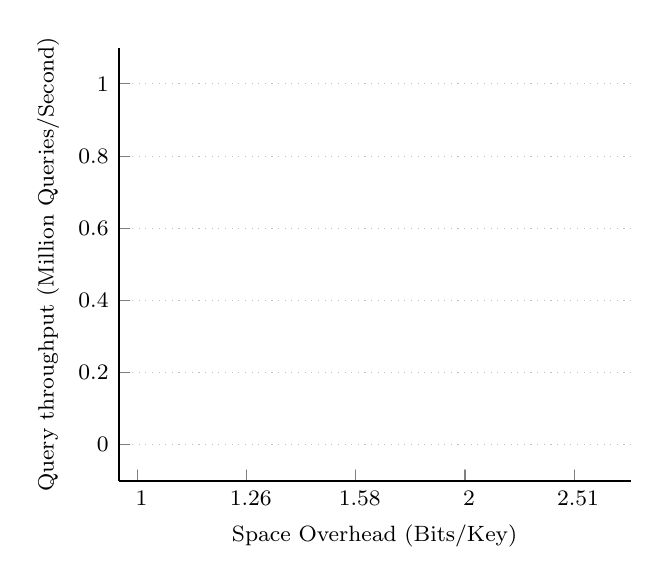
\begin{tikzpicture}
    \begin{axis}[
            ylabel={Query throughput (Million Queries/Second)},
            xlabel={Space Overhead (Bits/Key)},
            legend columns=4,
            xmode=log,
            patch,
            patch type=rectangle,
            shader=flat,
            xmin=0.015,
            xmax=5,
        ]
        % Each point in the dominance map is a rectangle going infinitely far to the right and bottom.
        % Sorting the draw order of these rectangles by the third dimension gives the dominance map.
        % The NULL values in the rectangle get filled with the actual measurements.
        % SQL DELETE FROM rectangle
        % SQL INSERT INTO rectangle VALUES (NULL,NULL),(10,NULL),(10,0),(NULL,0)

        %% MULTIPLOT(ptitle|attr|nolegend)
        %% SELECT
        %%   IFNULL(rectangleX, bitsPerElement-1.4427) AS x,
        %%   IFNULL(rectangleY, 0.001*numQueries/queryTimeMilliseconds) AS y,
        %%   store_attr || ",solid,mark=none,line width=0" AS attr,
        %%   store_name as ptitle
        %% FROM dominanceMap
        %% CROSS JOIN rectangle
        %% LEFT JOIN competitorNames ON name = store_code
        %% ORDER BY constructionTimeMilliseconds DESC
    \end{axis}
\end{tikzpicture}

\centering
\begin{tikzpicture}
    \ref*{legend}
\end{tikzpicture}

\end{document}

